\subsection{Outline of the finite reduction}\label{app:reduction-outline}

\Cref{sec:setting} produced a global minimizer of the control problem whose state stays in the
compact domain $\hstarstar$. This section shows that, after a change of origin in time, such a
minimizer has a control that takes only the three vertex values $\ee_0,\ee_1,\ee_2$, switching
finitely often in a period, and that it carries a Pontryagin lift with cost multiplier
$\lambda=-1$. The conclusion is \cref{thm:finite-normal}. Every later section starts from it.

The steps are the following. The maximum principle gives a lift $(\Lambda_1,\Lambda_R,\lambda)$ of
the minimizer, possibly abnormal ($\lambda=0$). The danger is the singular locus, where the
Hamiltonian does not depend on the control and the maximum condition gives no information. Near it
Hales and Vajjha find Fuller's system~\cite{HalesVajjha2024,Fuller1963}, whose optimal controls
switch infinitely often in finite time. A budget inequality, which uses only that the cost is at
most $\Aoct<\pi$, keeps every lift away from the singular locus in proportion to its size
(\cref{prop:clearance}). Away from the singular locus one vertex is excluded on each side of every
time (\cref{red:local-exclusion}). On an interval where one vertex is excluded the control runs
along an edge of the simplex, and an edge minimizer has at most four pieces
(\cref{prop:edge-bound}). Compactness of $[0,T]$ then gives finitely many pieces
(\cref{prop:finite-switches}). Merging equal neighbours and restarting the period at a genuine
switch gives a vertex representation (\cref{lem:word-reduction}), and for a lift of a trajectory
with a vertex representation the multiplier is nonzero (\cref{thm:normality}).

The order matters. The clearance and the switch count are homogeneous in
$(\lambda,\Lambda_1,\Lambda_R)$, so they hold for abnormal lifts as well as normal ones. The
normality argument, on the other hand, reads the costate at the finitely many switching times
and uses the twisted closing condition of the period. Finiteness is therefore proved first, for an
arbitrary lift, and normality afterwards.

\subsection{Pontryagin extremals}\label{red:extremals}

The maximum principle is applied to the problem of \cref{def:control-problem} with free terminal
time and with the closing conditions $g(0)=I$, $g(T)=R$, $X(T)=R^{-1}X(0)R$. Its conclusions, in
the form of Hales and Vajjha's Problem~6.7.1~\cite{HalesVajjha2024}, define the following object.

\begin{definition}[Pontryagin extremal]\label{def:pmp-extremal}
Let $(T,u,g,X)$ be a state trajectory (\cref{def:control-problem}) with $g(0)=I$, $g(T)=R$ and
$X(T)=R^{-1}X(0)R$. A \emph{Pontryagin lift} of it consists of two curves
$\Lambda_1,\Lambda_R\colon[0,T]\to\sltwo$ and a constant $\lambda\le0$, the \emph{cost
multiplier}, such that
\begin{enumerate}
\item $\ip{\Lambda_R(t)}{X(t)}=0$ and $(\lambda,\Lambda_1(t),\Lambda_R(t))\ne0$ for every
  $t\in[0,T]$;
\item $\Lambda_1$ and $\Lambda_R$ are absolutely continuous and satisfy, for almost every $t$,
  \begin{equation}\label{red:costate}
  \Lambda_1'=[\Lambda_1,X],\qquad
  \Lambda_R'=[P_u,\Lambda_R]-\ip{\Lambda_R}{P_u}[P_u,X]+[-\Lambda_1+\tfrac32\lambda J,X],
  \end{equation}
  with $P_u=Z_u/\ip{Z_u}{X}$ as in \cref{eq:state};
\item for almost every $t\in(0,T)$ the control $u(t)$ maximizes over $\UT$ the Hamiltonian
  \begin{equation}\label{red:hamiltonian}
  H(\Lambda_1,\Lambda_R,X;v)=\ip{\Lambda_1-\tfrac32\lambda J}{X}
  -\frac{\ip{\Lambda_R}{Z_v}}{\ip{X}{Z_v}},
  \end{equation}
  evaluated at $(\Lambda_1(t),\Lambda_R(t),X(t))$, and the maximum is $0$;
\item $\Lambda_1(T)=R^{-1}\Lambda_1(0)R$ and $\Lambda_R(T)=R^{-1}\Lambda_R(0)R$.
\end{enumerate}
The tuple $(T,u,g,X,\Lambda_1,\Lambda_R,\lambda)$ is a \emph{Pontryagin extremal}. It is \emph{normal} if $\lambda\ne0$ and
\emph{abnormal} if $\lambda=0$.
\end{definition}

Here $\Lambda_1$ is the costate of the frame, read in the left trivialization of $\SLtwo$, and
$\Lambda_R=[\Lambda_2,X]$ is the part of the costate of the state that the dynamics see. The
conditions are positively homogeneous in $(\Lambda_1,\Lambda_R,\lambda)$, so a normal lift can be
rescaled to $\lambda=-1$.

\begin{theorem}[Pontryagin lift]\label{thm:pmp-lift}
Every global minimizer $(T,u,g,X)$ of the control problem (\cref{def:global-minimizer}) has a
Pontryagin lift $(\Lambda_1,\Lambda_R,\lambda)$.
\end{theorem}

Hales and Vajjha use this statement in the proof of their Proposition~8.1.3. It follows from the
maximum principle with free terminal time~\cite{Pontryagin1962,AgrachevSachkov2004}, applied on the
open subset of $\R^{2\times2}\times\sltwo$ cut out by $\det g>0$ and the star inequalities, with
the costates read through the left trivialization. The nontriviality of the reduced costate
$(\lambda,\Lambda_1,\Lambda_R)$ needs a separate argument: if $\lambda=0$ and $\Lambda_1$,
$\Lambda_R$ vanish at one time, then $\Lambda_1\equiv0$ by the conservation law below, and the
equation for $\Lambda_R$ becomes linear and homogeneous, so $\Lambda_R\equiv0$.

Two consequences of the costate equations are used throughout. The first is the conservation law
of Hales and Vajjha's Corollary~6.5.3,
\begin{equation}\label{red:conservation}
\Lambda_1(t)=g(t)^{-1}\Lambda_1(0)\,g(t)\qquad(0\le t\le T)
\end{equation}. In particular $\det\Lambda_1$ is constant. The second
concerns the three \emph{vertex Hamiltonians} $H_i(t)=H(\Lambda_1(t),\Lambda_R(t),X(t);\ee_i)$.
The denominator $-\ip{X}{Z_v}$ is positive and affine in $v$, and
$-\ip{X}{Z_v}\bigl(H(\cdot\,;v)-c\bigr)$ is affine in $v$ for every constant $c$. So the maximum of
$H$ over the simplex is attained at a vertex, and a vertex carrying positive weight in a maximizing
control is itself maximizing.

\begin{lemma}[Vertex Hamiltonians]\label{lem:vertex-hamiltonians}
For a Pontryagin extremal the vertex Hamiltonians $H_0,H_1,H_2$ are continuous on $[0,T]$, and at
every $t\in[0,T]$, not only almost every $t$, all three are $\le0$ and one of them is $0$.
\end{lemma}

\begin{proof}
Continuity holds because $X$, $\Lambda_1$, $\Lambda_R$ are continuous and $\ip{X}{Z_{\ee_i}}<0$ on
star states. By the maximum condition, $\max_iH_i(t)=0$ for almost every $t$, hence for every $t$
by continuity of $\max_iH_i$.
\end{proof}

\Cref{fig:red-hamiltonians} shows the three vertex Hamiltonians along the smoothed octagon's
period, for its normal lift.

\begin{figure}[htbp]
\centering
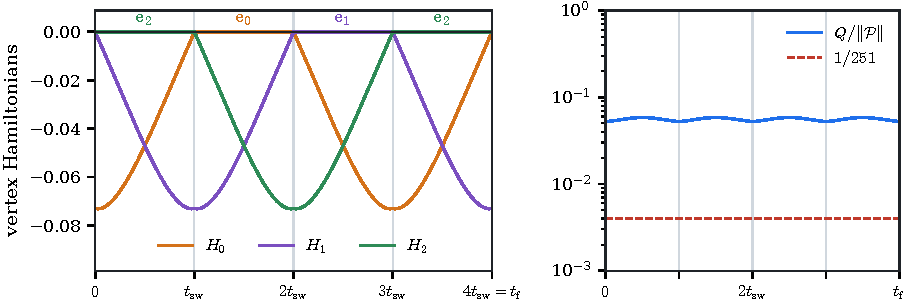
\includegraphics[width=\textwidth]{figures/fig-reduction-hamiltonians.pdf}
\caption{The normal Pontryagin lift ($\lambda=-1$) of the smoothed octagon's trajectory over one
period $[0,\tf]$, with control word $\ee_2\ee_0\ee_1\ee_2$ and switching time $\tsw=\tf/4$; the
lift is that of Hales and Vajjha's Theorem~7.5.1~\cite{HalesVajjha2024}, integrated numerically.
Left: the vertex Hamiltonians $H_0,H_1,H_2$. All three are $\le0$, the vertex of the current piece
has $H_i=0$, and at each switch the incoming vertex reaches $0$. Right: the ratio
$Q/\norm{\mathcal P}$ of \cref{prop:clearance}, on a logarithmic scale. It stays above the
uniform positive lower bound supplied by that proposition. The computation
confirms the closing conditions $\Lambda_1(\tf)=R^{-1}\Lambda_1(0)R$ and
$\Lambda_R(\tf)=R^{-1}\Lambda_R(0)R$ and every property stated here.}
\label{fig:red-hamiltonians}
\end{figure}

\runin{The singular locus.} If the three vertex Hamiltonians are equal at some time, then the maximum
condition at that time says nothing about the control. Hales and Vajjha's Lemma~8.2.1 identifies
when this happens.

\begin{lemma}[Singular locus]\label{red:singular-locus}
Let $X$ be a star state and $\Lambda_R$ traceless with $\ip{\Lambda_R}{X}=0$. Then
$H(\Lambda_1,\Lambda_R,X;\ee_0)=H(\Lambda_1,\Lambda_R,X;\ee_1)=H(\Lambda_1,\Lambda_R,X;\ee_2)$ if
and only if $\Lambda_R=0$. If
$\Lambda_R\ne0$, there is a coordinate $i$ such that $v_i=0$ for every control $v$ maximizing $H$
over $\UT$.
\end{lemma}

So all three vertices tie at a time where $\Lambda_R=0$; if the Hamiltonian also vanishes there,
then $\ip{\Lambda_1-\frac32\lambda J}{X}=0$. The \emph{singular locus} is the set of costates with
$\Lambda_1=\frac32\lambda J$ and $\Lambda_R=0$; there $H(\cdot\,;v)=0$ for every control $v$. Put
\[
A=\Lambda_1-\tfrac32\lambda J,\qquad
\norm{\mathcal P}^2=\lambda^2+\norm{\Lambda_1}^2+\norm{\Lambda_R}^2,\qquad
Q^2=\norm{A}^2+\norm{\Lambda_R}^2,
\]
with Frobenius norms. Here $\mathcal P=(\lambda,\Lambda_1,\Lambda_R)$ is the extended covector,
and $Q$ is its distance from the singular locus.

\subsection{Singular clearance}\label{red:clearance-sec}

The singular locus cannot be excluded by local considerations; the argument uses the whole
period and its cost. Write $\omega(Y)=-\frac12\ip{J}{Y}$. For a star state $\omega(Y)\ge1$, and
the cost density is $-\frac32\ip{J}{X}=3\omega(X)$, so $\cost(T,X)=3\int_0^T\omega(X)$. For a
frame $h$ with $\det h=1$ put $\omega_R(h,Y)=\omega(hYh^{-1})$, the same quantity for the state
seen in the fixed frame.

\begin{lemma}[Winding]\label{red:winding}
For every admissible trajectory $(T,u,h,Y)$, with $h(0)=I$ and $h(T)=R$,
\[
\int_0^T\bigl(\omega(Y)+\omega_R(h,Y)\bigr)\,\dd t\ \ge\ \frac{2\pi}3.
\]
\end{lemma}

\begin{proof}
Write $\zeta(h)=\frac12(h_{00}+h_{11})+\frac i2(h_{10}-h_{01})\in\mathbb C$, the coefficient of
$h$ on the rotations. Since $\det h=1$, $\abs{\zeta(h)}\ge1$, and a direct computation gives
$\omega(Y)+\omega_R(h,Y)=2\operatorname{Im}\bigl(\overline{\zeta}\,\zeta'\bigr)$ along $h'=hY$. Let $L(t)=\int_0^t\zeta'/\zeta$, so that $\zeta=e^{L}$. Then
$\operatorname{Im}(\zeta'/\zeta)=(\omega+\omega_R)/(2\abs\zeta^2)>0$, and
$\zeta(T)=\zeta(R)=e^{i\pi/3}$ forces $\operatorname{Im}L(T)\in\frac\pi3+2\pi\Z$; being positive,
it is at least $\pi/3$. Since $\abs\zeta\ge1$,
$\int_0^T(\omega+\omega_R)=2\int_0^T\abs\zeta^2\operatorname{Im}(\zeta'/\zeta)
\ge2\operatorname{Im}L(T)\ge2\pi/3$.
\end{proof}

The second ingredient is pointwise: at a star state the control $u^*$ with $P_{u^*}=-X/2$ lies
in the simplex and has $H(u^*)=\ip{A}{X}$, so the maximum condition gives $\ip{A}{X}\le0$. The
weights of $u^*$ also bound $\Lambda_R$.

\begin{lemma}[Equilibrium inequality]\label{red:equilibrium}
Let $X$ be a star state, $\Lambda_R$ traceless with $\ip{\Lambda_R}{X}=0$, and suppose that every
vertex Hamiltonian at $(\Lambda_1,\Lambda_R,X)$ is $\le0$. Then $\ip{A}{X}\le0$. On each compact
set of star states there is a constant $C$ such that
$\norm{\Lambda_R}\le C\bigl(-\ip{A}{X}\bigr)$.
\end{lemma}

\begin{proof}
With $\varsigma_i=\sqrt3\ip{\Lambda_R}{Z_{\ee_i}}$ and the margins $p_i$ of \cref{lem:margins}, the
vertex Hamiltonians are $H_i=\ip{A}{X}+\varsigma_i/p_i$. The weights $\vartheta_i=p_i(p_j+p_k)/8$,
$\{i,j,k\}=\{0,1,2\}$, sum to $1$ by $p_0p_1+p_1p_2+p_2p_0=4$, and
$\sum_i\vartheta_i\varsigma_i/p_i=\frac18\sum_i(p_j+p_k)\varsigma_i
=\frac12\ip{\Lambda_R}{X}=0$. Hence $\ip{A}{X}=\sum_i\vartheta_iH_i\le0$. Put $m=-\ip{A}{X}\ge0$. From
$H_i\le0$, $(p_j+p_k)\varsigma_i\le8m\vartheta_i$. Since the three products
$(p_j+p_k)\varsigma_i$ sum to zero, each is at least the negative of the upper bounds for the
other two, hence at least $-8m(1-\vartheta_i)\ge-8m$; its upper bound is also at most $8m$.
On a compact set of star states every $p_j+p_k$ has a positive lower bound. Thus every
$\abs{\varsigma_i}$ is bounded by a fixed multiple of $m$. The matrices $Z_{\ee_i}$ span
$\sltwo$, and the trace form on $\sltwo$ is nondegenerate, so the linear map
$\Lambda_R\mapsto(\varsigma_0,\varsigma_1,\varsigma_2)$ is invertible. Its inverse has bounded
norm, proving the assertion.
\end{proof}

Only the strict gap between the octagon's cost and the circular cost enters the next estimate.
For $0\le c<\pi$ write
\[
 b(c)=\frac{2\pi-c}{3(\pi-c)},\qquad b_{\mathrm{oct}}=b(\Aoct).
\]
The function $b$ is increasing, and it is finite precisely while the cost stays below $\pi$.

\begin{proposition}[Budget inequality]\label{red:budget}
Let $(T,u,h,Y)$ be admissible with $\cost(T,Y)\le\Aoct$, let $M\in\R^{2\times2}$ and $\mu\in\R$, and
suppose $\ip{h(t)^{-1}Mh(t)+\frac32\mu J}{Y(t)}\le0$ for $t\in[0,T]$. Then
$\mu\le b_{\mathrm{oct}}\,\norm{M+\frac32\mu J}$. Consequently every Pontryagin
extremal with cost at most $\Aoct$ satisfies
\[
\abs\lambda\le b_{\mathrm{oct}}\,\bigl\lVert\Lambda_1(t)-\tfrac32\lambda J\bigr\rVert
\qquad(0\le t\le T).
\]
\end{proposition}

\begin{proof}
Put $A_0=M+\frac32\mu J$, $a_0=\norm{A_0}$ and $V=hYh^{-1}$. The hypothesis reads
$\ip{A_0}{V}+3\mu\,\omega_R\le3\mu\,\omega$. By the Cauchy--Schwarz inequality and
$\norm{V}^2=4\omega_R^2-2$, $\ip{A_0}{V}\ge-2a_0\omega_R$, so
$(3\mu-2a_0)\omega_R\le3\mu\,\omega$ pointwise. Let $c=\cost(T,Y)$,
$I=\int\omega=c/3$ and $I_R=\int\omega_R$. If $3\mu\le2a_0$, then
$\mu\le2a_0/3\le b(c)a_0$. Otherwise $3\mu-2a_0>0$, so integrating and using
$I_R\ge2\pi/3-I$ from \cref{red:winding} gives
\[
 (3\mu-2a_0)(2\pi-c)\le3\mu c,
 \qquad\text{hence}\qquad
 3\mu(\pi-c)\le a_0(2\pi-c).
\]
Since $c\le\Aoct<\pi$, division gives $\mu\le b(c)a_0\le b_{\mathrm{oct}}a_0$.
For the consequence, rebase
the twisted extension of the extremal at $t$ (\cref{red:rebase}). The rebased trajectory is
admissible with the same cost, its costate at time $0$ is $\Lambda_1(t)$ by \cref{red:conservation},
and \cref{red:equilibrium} gives the hypothesis with $M=\Lambda_1(t)$ and $\mu=-\lambda$.
\end{proof}

The gap $\pi-\Aoct>0$ is what makes the budget effective. It bounds the
multiplier by the distance $\norm{A}$ from $\Lambda_1$ to $\frac32\lambda J$; adding
$\norm{\Lambda_R}$ gives the clearance.

Put
\[
 c_{\mathrm{oct}}=
 \sqrt{b_{\mathrm{oct}}^2+\bigl(1+3b_{\mathrm{oct}}/\sqrt2\bigr)^2}.
\]

\begin{proposition}[Singular clearance]\label{prop:clearance}
Let $(T,u,g,X,\Lambda_1,\Lambda_R,\lambda)$ be a Pontryagin extremal, normal or abnormal, with
$\cost(T,X)\le\Aoct$ and $X(t)\in\hstarstar$ for $t\in[0,T]$. Then
\[
\norm{\mathcal P(t)}\le c_{\mathrm{oct}}\,Q(t)\qquad(0\le t\le T).
\]
In particular $Q(t)>0$ for every $t$: the costate never meets the singular locus.
\end{proposition}

\begin{proof}
Write $\Lambda_1=A+\frac32\lambda J$. Since $\norm{J}=\sqrt2$, the triangle inequality and
\cref{red:budget} give
\[
 \norm{\Lambda_1}\le\norm{A}+\frac3{\sqrt2}\abs\lambda
 \le\bigl(1+3b_{\mathrm{oct}}/\sqrt2\bigr)\norm{A}.
\]
Consequently
$\norm{\mathcal P}^2\le c_{\mathrm{oct}}^2\norm{A}^2+\norm{\Lambda_R}^2
\le c_{\mathrm{oct}}^2Q^2$, since $c_{\mathrm{oct}}>1$.
The positivity of $Q$ follows from the nontriviality
$\norm{\mathcal P}>0$.
\end{proof}

\begin{remark}\label{red:clearance-remark}
These estimates are uniform on each compact set $K$ of star states. By
\cref{red:equilibrium} and the boundedness of $\norm X$ on $K$, there is $D_K\ge0$ such that
$\norm{\Lambda_R}^2\le D_K\norm A^2$. Put $F=2e^{2\Aoct/3}$. Along $g'=gX$,
\[
 \frac{\dd}{\dd t}\norm g^2=2\tr(Xg^{\mathsf T}g)
 \le2\omega(X)\norm g^2,
\]
so Gronwall's inequality gives $\norm{g(t)}^2\le F$. Since
$\norm{g^{-1}}=\norm g$ for $\det g=1$, spatial conservation
(\cref{red:conservation}) bounds $\norm{\Lambda_1(t)}^2$ by
$F^2\norm{\Lambda_1(0)}^2$ and conversely. Together with
$\norm A^2\le2\norm{\Lambda_1}^2+9\lambda^2$, this yields
\[
 G_K^{-1}\norm{\mathcal P(0)}^2\le\norm{\mathcal P(t)}^2
 \le G_K\norm{\mathcal P(0)}^2,
 \qquad G_K=(1+9D_K)+(1+2D_K)F^2.
\]
The constant depends only on $K$ and $\Aoct$.
\end{remark}

\subsection{The edge bound}\label{red:edge-sec}

Suppose that on a time interval one coordinate of the control vanishes almost everywhere, say
$u_0=0$. The trajectory then runs along the edge of the simplex opposite $\ee_0$, and the control is
determined by one number $v=u_1\in[0,1]$. A priori $v$ could still alternate between the two
remaining vertices infinitely often. The following bound excludes this for a global minimizer.

\begin{proposition}[Edge bound]\label{prop:edge-bound}
Let $(T,u,g,X)$ be a global minimizer, $0\le t_0<t_1\le T$, and $j\in\{0,1,2\}$ with $u_j=0$ almost
everywhere on $(t_0,t_1)$. Then on $[t_0,t_1]$ the control is almost everywhere a concatenation of
at most four constant vertex pieces of positive length.
\end{proposition}

\begin{proof}
Relabeling by a power of $R$ (\cref{red:rebase}) moves the missing vertex to $j=0$ and keeps
minimality. On the edge, a star state $X=\bigl(\begin{smallmatrix}a&b\\c&-a\end{smallmatrix}\bigr)$
has $b=-(1+a^2)/c$, and the star inequalities read $c>0$, $3a^2<c^2<3(1+a^2)$. With
$u=(0,v,1-v)$ and $\alpha=(2v-1)/\sqrt3$, the state equation becomes the control system
\[
a'=\frac{c}{c-3\alpha a},\qquad c'=\frac{3\alpha c}{c-3\alpha a},\qquad s'=c,
\]
in the state $(a,c,s)$, $s=\int c$, with cost density $\frac32\bigl(c+(1+a^2)/c\bigr)$. The frame is recovered from $x=a/c$ and $s$. Replacing the segment $[t_0,t_1]$ of the minimizer by any
edge trajectory with the same end states and end frames, and translating the rest of the
trajectory in time, gives an admissible trajectory whose cost changes by the difference of the
segment costs. Since competitors with any terminal time are
allowed, the segment minimizes the edge cost among edge trajectories with its end points and free
duration.

The maximum principle with free time applies to this system on the open set given by the star
inequalities. It gives a multiplier $\nu\le0$ and a covector $p=(p_a,p_c,p_s)$ with
$(\nu,p(t))\ne0$ and $H=0$, and $p_s$ is constant since the system does not depend on $s$. The
derivative of the Hamiltonian in $\alpha$ is $3c\,\varsigma/(c-3\alpha a)^2$ with the
\emph{switching function} $\varsigma=ap_a+cp_c$, so $v=1$ where $\varsigma>0$ and $v=0$ where
$\varsigma<0$. The adjoint equation, the homogeneity of the field in $(a,c)$ and $H=0$ give
\[
\varsigma'=-c\,\bigl(2p_s+3\nu(1+x^2)\bigr),\qquad x=a/c,\quad x'=1/c>0.
\]
Since $x$ is strictly increasing, the quadratic $2p_s+3\nu(1+x^2)$ vanishes at most twice in time
unless $\nu=p_s=0$; then $\varsigma$ has at most three zeros by Rolle's theorem, and the control
has at most four constant pieces. If $\nu=p_s=0$, then $\varsigma$ is constant, and it is nonzero,
because $\varsigma=0$ and $H=0$ would force $p=0$.
\end{proof}

\subsection{Finitely many switches}\label{red:switch-sec}

\begin{lemma}[Local exclusion of a vertex]\label{red:local-exclusion}
Let $(T,u,g,X,\Lambda_1,\Lambda_R,\lambda)$ be a Pontryagin extremal with $X(t)\in\hstarstar$ on
$[0,T]$, and let $t_0\in[0,T]$ with $Q(t_0)>0$. There are $\delta>0$ and vertices $j,k$ such that
$H_j<0$ on $(t_0,t_0+\delta)\cap[0,T]$ and $H_k<0$ on $(t_0-\delta,t_0)\cap[0,T]$.
\end{lemma}

\begin{proof}
If $H_i(t_0)<0$ for some $i$, continuity gives the claim with $j=k=i$. Otherwise all three vertex
Hamiltonians vanish at $t_0$ (\cref{lem:vertex-hamiltonians}), so $\Lambda_R(t_0)=0$ by
\cref{red:singular-locus} and $\ip{A}{X}=0$ there. Then $Q(t_0)>0$ gives $A(t_0)\ne0$, and
$b=[X(t_0),A(t_0)]\ne0$, since a traceless matrix commuting with $X$ is a multiple of $X$ and
$\ip{X}{X}=-2$. The control-dependent terms of \cref{red:costate} are $O(\norm{\Lambda_R})$, so
$\Lambda_R'(t_0)=b$, and $h_i=\ip{\Lambda_R}{Z_{\ee_i}}/\ip{X}{Z_{\ee_i}}$ has derivative
$c_i=\ip{b}{Z_{\ee_i}}/\ip{X}{Z_{\ee_i}}$ at $t_0$. As $b$ is traceless and orthogonal to $X$,
\cref{red:singular-locus} applied to $b$ shows that the $c_i$ are not all equal. If $c_k<c_j$, then
$H_j-H_k=h_k-h_j$ vanishes at $t_0$ with negative derivative, so $H_j<H_k\le0$ just after $t_0$ and
$H_k<H_j\le0$ just before.
\end{proof}

Where $H_j<0$ on an interval, the coordinate $u_j$ of the control vanishes almost everywhere there,
because a vertex with positive weight in a maximizing control is maximizing. So the edge bound applies on both sides of $t_0$.

\begin{proposition}[Finitely many switches]\label{prop:finite-switches}
Let $(T,u,g,X,\Lambda_1,\Lambda_R,\lambda)$ be a Pontryagin extremal with $\cost(T,X)\le\Aoct$ and
$X(t)\in\hstarstar$ on $[0,T]$, satisfying the clearance of \cref{prop:clearance}, and whose control
has the property of \cref{prop:edge-bound}. Then there is $n$ such that on $[0,T]$ the control is
almost everywhere a concatenation of $n$ constant vertex pieces of positive length.
\end{proposition}

\begin{proof}
By \cref{prop:clearance}, $Q(t_0)>0$ at every $t_0$. \Cref{red:local-exclusion} and the edge bound
give, around each $t_0$, a $\delta>0$ such that every subinterval of $[0,T]$ inside
$(t_0-\delta,t_0+\delta)$ has a finite vertex description: on the part after $t_0$ the vertex $j$
is missing and \cref{prop:edge-bound} gives at most four pieces, on the part before $t_0$ the vertex
$k$ is missing, and the two descriptions concatenate at $t_0$. A Lebesgue number of this cover of
the compact interval $[0,T]$ and induction along a uniform partition give a finite description of
$[0,T]$.
\end{proof}

\subsection{Vertex representations and rebasing}\label{red:rebase}

\begin{definition}[Vertex representation]\label{def:vertex-representation}
A \emph{vertex representation} of a control $u$ on $[0,T]$ consists of an integer $N\ge1$, a
strictly increasing sequence $(\tau_k)_{k\in\Z}$ of \emph{switching times} with $\tau_0=0$ and
$\tau_{k+N}=\tau_k+T$, and \emph{labels} $i_k\in\Z/3$ with $i_{k+N}=i_k+1$ and $i_{k+1}\ne i_k$ for
every $k\in\Z$, such that for $0\le k<N$ the control equals $\ee_{i_k}$ almost everywhere on
$(\tau_k,\tau_{k+1})$. The interval $(\tau_k,\tau_{k+1})$ is the
$k$-th \emph{piece}, and $N$ is the number of pieces of the period.
\end{definition}

\begin{definition}[Normal period]\label{def:normal-period}
A \emph{normal period} is a Pontryagin extremal $(T,u,g,X,\Lambda_1,\Lambda_R,\lambda)$ with
$\lambda=-1$, together with a vertex representation of its control $u$. It is
\emph{competitive} if $\cost(T,X)\le\Aoct$, and it lies in the
compact domain if $X(t)\in\hstarstar$ for $t\in[0,T]$. The
\emph{active margin} of the $k$-th piece is $a_k=p_{i_k}(X(\tau_k))$, with $k$ read modulo $N$.
\end{definition}

The pieces of \cref{prop:finite-switches} may have equal neighbouring labels, and the cut at $t=0$
need not be a switch. Both are repaired by extending the trajectory periodically. The \emph{twisted
extension} of an admissible trajectory $(T,u,g,X)$ is defined for $t\ge0$ by
\[
G(t)=g(t-nT)R^n,\qquad Y(t)=R^{-n}X(t-nT)R^n,\qquad n=\lfloor t/T\rfloor,
\]
and with the control $v(t)$ equal to $u(t-nT)$ with its coordinates shifted $n$ times, so that
the vertex $\ee_i$ becomes $\ee_{i+n}$ and $Z_{v(t+T)}=R^{-1}Z_{v(t)}R$. The extension satisfies the state equations
on every interval $[0,nT]$. The trajectory \emph{rebased} at $s\in[0,T)$ is, for $0\le t\le T$,
\[
\hat g(t)=G(s)^{-1}G(s+t),\qquad \hat X(t)=Y(s+t),\qquad \hat u(t)=v(s+t).
\]
It is again admissible, and it has the same cost because $J$ commutes with $R$; so a rebased global
minimizer is a global minimizer. Similarly the
\emph{relabeling} $(g,X)\mapsto(R^{-r}gR^r,R^{-r}XR^r)$, with the control coordinates shifted $r$
times, preserves admissibility and cost.



In a vertex representation (\cref{def:vertex-representation}), the condition $i_{k+1}\ne i_k$ for every $k$, including $k=N-1$, says that equal neighbours have
been merged also across the seam $t=T$, where the label after the last piece is $i_N=i_0+1$.

\begin{lemma}[Merging and rebasing]\label{lem:word-reduction}
If on $[0,T]$ the control $u$ is almost everywhere a concatenation of $n$ vertex pieces, there is
$s\in[0,T)$ such that the rebased control $\hat u$ has a vertex representation with $N\le n$ pieces.
\end{lemma}

\begin{proof}
Extend the pieces by the twist to a bi-infinite sequence with $\tau_{k+n}=\tau_k+T$ and labels
$l_{k+n}=l_k+1$. Call $\tau_k$ a genuine switch if $l_k\ne l_{k-1}$. The increments
$l_k-l_{k-1}$ over one period sum to $1\ne0$ in $\Z/3$, so some increment is nonzero, and a genuine
switch $s=\tau_{k_0}$ lies in $[0,T)$. Merge the pieces of $[s,s+T]$ with equal neighbouring
labels, shift by $-s$, and extend the reduced word to $\Z$ by the twist; the seam condition is the
genuine switch at $s$.
\end{proof}

\subsection{Normality}\label{red:normal-sec}

Recall the normal periods of \cref{def:normal-period}.

\begin{theorem}[Normality]\label{thm:normality}
Let $(T,u,g,X)$ be a global minimizer with a Pontryagin lift $(\Lambda_1,\Lambda_R,\lambda)$, and
suppose that $u$ has a vertex representation. Then $\lambda<0$, and
$(\Lambda_1,\Lambda_R,\lambda)/(-\lambda)$ is a Pontryagin lift with multiplier $-1$.
\end{theorem}

The proof reads an abnormal costate at the switching times, in coordinates in which every piece
acts by an explicit linear map, and derives a contradiction with the twisted closing condition.

\runin{Coordinates.} For $M\in\sltwo$ put $\mu_j(M)=\sqrt3\ip{M}{Z_{\ee_j}}$, so that the margins
are $p_j=-\mu_j(X)$. With $\lambda=0$ put
\[
a=-X\Lambda_1X,\qquad b=\Lambda_R+2\Lambda_1+\ip{\Lambda_1}{X}X.
\]
Using $X^2=-I$ and $X\Lambda X=\ip{\Lambda}{X}X+\Lambda$ one finds
$p_jH_j=2\mu_j(a)+\mu_j(b)$; this is the abnormal
analogue of the switching functions $\chi_j$ of \cref{def:costate-coordinates}. Moreover
$\ip{b}{X}=\ip{\Lambda_R}{X}=0$, and $(a,b)=0$ only if $(\Lambda_1,\Lambda_R)=0$. For a label $i$
and $q>0$ let $L_i(q)$ be the linear map of $\R^3$ that fixes the coordinate $i$ and sends
\[
v_{i+1}\mapsto(v_i+v_{i+1})q-v_i,\qquad v_{i-1}\mapsto(v_i+v_{i-1})/q-v_i,
\]
the one-arc margin map of \cref{lem:one-arc}.

\begin{lemma}[Abnormal transport]\label{red:abnormal-transport}
Let the extremal have $\lambda=0$, and let $u=\ee_i$ almost everywhere on a piece $(s_0,s_1)$, with
$q=\exp\bigl(2(s_1-s_0)/p_i(X(s_0))\bigr)$. Then $H_i(s_0)=0$; the margins and the coordinates
$\mu(b)$ at $s_1$ are those at $s_0$ transformed by $L_i(q)$; and the coordinates $\mu(a)$ are
transformed by $L_i(q^2)$.
\end{lemma}

\begin{proof}
Write $S_j=\sqrt3Z_{\ee_j}$. On the piece $P_u=-S_i/p_i$ is constant, since the active margin
$p_i$ is constant. The state, $a$ and $b$ satisfy $f'=\kappa[P_u,f]$ with $\kappa=1,2,1$
respectively; for $b$ this uses that the active vertex Hamiltonian vanishes on the piece. The
relation $[S_i,S_{i+1}]=2(S_i+S_{i+1})$ and the invariance of the trace form make $\mu_i(f)$
constant and multiply $\mu_i(f)+\mu_{i\pm1}(f)$ by $q^{\pm\kappa}$.
\end{proof}

\begin{proof}[Proof of \cref{thm:normality}]
Suppose $\lambda=0$. Continue the lift through the seams by the twist, using the closing conditions
$X(T)=R^{-1}X(0)R$, $\Lambda_1(T)=R^{-1}\Lambda_1(0)R$, $\Lambda_R(T)=R^{-1}\Lambda_R(0)R$, which
relabel the coordinates. At the switching times $\tau_k$, $k\ge0$, this gives labels $i_k$ with
$i_{k+1}\ne i_k$ and $i_{k+N}=i_k+1$, factors $q_k>1$, positive margins, and coordinates
$\alpha_k=\mu(a(\tau_k))$, $\beta_k=\mu(b(\tau_k))$, related by \cref{red:abnormal-transport}, with
$\sum_{j\ne l}\beta_{k,j}p_l=0$, the active quantity
$\chi_{i_k}(k)=2\alpha_{k,i_k}+\beta_{k,i_k}=0$, $\chi_j(k)=2\alpha_{k,j}+\beta_{k,j}\le0$ for all
$j$ by \cref{lem:vertex-hamiltonians}, and $(\alpha_k,\beta_k)\ne0$. Four facts about such a sequence follow.
\begin{enumerate}
\item No piece has a triple tie, $\chi_0=\chi_1=\chi_2=0$, at both of its ends. Indeed, for $j\ne i=i_k$ the pair sums
  $x=\alpha_i+\alpha_j$ and $y=\beta_i+\beta_j$ are multiplied by $\varrho^2$ and $\varrho$ along the
  piece, $\varrho\in\{q_k,q_k^{-1}\}$. The ties $2x+y=0$ at both ends give $x(\varrho^2-\varrho)=0$,
  so $x=y=0$. Hence $\beta_i=-2\alpha_i$ and $\beta_j=2\alpha_i$ for $j\ne i$, and the orthogonality
  relation becomes $4\alpha_ip_i=0$. Then $\alpha=\beta=0$, against nontriviality.
\item If three consecutive pieces carry labels $i,j,i$, then $\chi_j$ vanishes at the start of the
  first and at the end of the third.
\item No three consecutive switches have the same sign: the
  inequalities $\chi\le0$ for the missing vertex at the two inner switches, combined with the
  transports, force triple ties at both ends of the middle piece, against~(1).
\item From the second switch on, neighbouring switches have opposite signs, that is,
  $i_{k+2}=i_k$ for $k\ge1$. This follows from~(1)--(3).
\end{enumerate}
By~(4), $i_{1+2N}=i_1$. By the twist, $i_{1+2N}=i_{1+N}+1=i_1+2$. Since $2\ne0$ in $\Z/3$, this is
a contradiction.
\end{proof}

The argument does not use the minimality of $(T,u,g,X)$: an abnormal lift of any trajectory with a
vertex representation contradicts the twisted closing condition.

\subsection{The finite normal representation}\label{red:assembly}

\begin{theorem}[Finite normal representation]\label{thm:finite-normal}
Let $(T,u,g,X)$ be a global minimizer of the control problem. There are a normal period
$(T,\hat u,\hat g,\hat X,\Lambda_1,\Lambda_R,-1)$, with a vertex representation of $\hat u$, and a
time $s\in[0,T)$ such that
\begin{enumerate}
\item $\hat g(t)=G(s)^{-1}G(s+t)$ and $\hat X(t)=Y(s+t)$ for $t\in[0,T]$, where $(G,Y)$ is the
  twisted extension of $(g,X)$;
\item $\cost(T,\hat X)=\cost(T,X)$, and $(T,\hat u,\hat g,\hat X)$ is a global minimizer;
\item $\hat X(t)\in\hstarstar$ for every $t\in[0,T]$.
\end{enumerate}
In particular the period is competitive,
$\cost(T,\hat X)\le\Aoct$.
\end{theorem}

\begin{proof}[Proof of \cref{thm:finite-normal}]
The state of the minimizer stays in $\hstarstar$ (\cref{thm:compact-domain}), and its cost is at
most $\Aoct$ since the octagon is a competitor. Take a Pontryagin lift (\cref{thm:pmp-lift}); it may
be abnormal. It satisfies the clearance (\cref{prop:clearance}), and the minimizer has the edge
property (\cref{prop:edge-bound}), so its control is a finite concatenation of vertex pieces
(\cref{prop:finite-switches}). Merge and rebase at a genuine switch $s$ (\cref{lem:word-reduction}).
The rebased trajectory is a global minimizer with the same cost (\cref{red:rebase}), so
\cref{thm:pmp-lift} applies to it directly; \cref{thm:normality} makes the new lift normal and
rescales it to $\lambda=-1$, and \cref{thm:compact-domain} applies to the rebased minimizer as
well.
\end{proof}

No costate is transported through the rebasing: the lift of the rebased minimizer is taken afresh,
which the minimality of the rebased trajectory allows. The theorem keeps the actual minimizer, with
its own frame and state, only restarted at $s$; the equality case of \cref{sec:equality} needs
this. From \cref{sec:periods} on, the hatted period is written $(T,u,g,X)$ again, with switching
times $\tau_k$, labels $i_k$ and active margins $a_k$.
